\documentclass{article}
\usepackage{arxiv}

\usepackage[utf8]{inputenc}
\usepackage[english, russian]{babel}
\usepackage[T1]{fontenc}
\usepackage{url}
\usepackage{booktabs}
\usepackage{amsfonts}
\usepackage{nicefrac}
\usepackage{microtype}
\usepackage{lipsum}
\usepackage{graphicx}
\usepackage{natbib}
\usepackage{doi}
\usepackage{amsmath} 



\title{Neural SDE: phase trajectories of SDE in the action}

\author{ Papay Ivan\\
	\texttt{papai.id@phystech.edu} \\
	%% examples of more authors
	\And
	Vladimirov Eduard \\
 \texttt{vladimirov.ea@phystech.edu} \\
 \And
	Strijov Vadim \\
 \texttt{strijov@phystech.edu} \\
	%% \AND
	%% Coauthor \\
	%% Affiliation \\
	%% Address \\
	%% \texttt{email} \\
	%% \And
	%% Coauthor \\
	%% Affiliation \\
	%% Address \\
	%% \texttt{email} \\
	%% \And
	%% Coauthor \\
	%% Affiliation \\
	%% Address \\
	%% \texttt{email} \\
}
\date{2024 год}

%%\renewcommand{\shorttitle}{\textit{arXiv} Template}

%%% Add PDF metadata to help others organize their library
%%% Once the PDF is generated, you can check the metadata with
%%% $ pdfinfo template.pdf
%\hypersetup{
%pdftitle={A template for the arxiv style},
%pdfsubject={q-bio.NC, q-bio.QM},
%pdfauthor={David S.~Hippocampus, Elias D.~Striatum},
%pdfkeywords={First keyword, Second keyword, More},
%}
\usepackage{algorithm}
\usepackage{algpseudocode}
\begin{document}

\maketitle

\begin{Abstract}
    Данная статья предлагает развить математический аппарат, на котором строится модель Neural SDE. В ней рассмотрено, как вычисление фазовых траекторий стохастических дифференциальных уравнений обеспечивает качественный прогноз аномалий во временном ряду. Таким образом, это предоставит как возможность эффективнее бороться с шумами, так и, в частности, полезный инструмент для упреждения появления так называемых `черных лебедей` - резких перемен поведения временных рядов, как случайных процессов. Подобного рода аномалии способны нарушить корректную работу Neural SDE в виду высокой корреляции элементов анализируемой выборки между собой.
\end{Abstract}


\keywords{SDE \and Stratonovich integral \and More}

\section{Введение}

   \par Сбор данных и подготовка их к последующей обработке являются одной из важнейших задач машинного обучения. Не всегда исследователь может гарантировать их целостность и корректность, ведь для тренировки модели чаще всего требуются выборки из тысяч, а то и десятков тысяч элементов --- не удивительно, что в данных допускается наличие шума, влияющего на работу обученной модели. Эта задача остаётся актуальной и для временных рядов. Нужно, имея данные для начала временного ряда, проверить: возможно ли предсказать его на некотором горизонте так, что это предсказание будет точным, и не сломает ли это природу текущего временного ряда в вероятностном смысле?
   \par В данной работе предполагается, что природа данных стохастическая. Входная выборка представляет из себя данные о некоем дискретном случайном процессе. От дискретного процесса корректно будет перейти к непрерывному в силу того факта, что он порождается сигма-алгеброй из конечномерных распределений, которые реально апроксимировать с помощью данных, предоставленных для обучения модели.
   \par Под данными имеются в виду значения n-мерного случайного процесса в фиксированном конечном множестве точек, которые необходимо будет сжать посредством CCA + CCM~(Convergent-Cross Mapping)[6]. В таком случае в качестве варианта апроксимации полученного одномерного временного ряда предлагается взять метод приближения обыкновенными дифференциальными уравнениями, от которых затем уже перейти к стохастическим.
   \par Сама идея использования обыкновенных дифференциальных уравнений~(`ОДУ`) не нова[1]. Так, примерно с 2017-го года она была использована[2] для создания и теоретического обоснования корректности работы модели Neural ODE. Тем не менее, такой метод был всё ещё слаб в робастном смысле[2]: был уязвим к состязательным атакам. Модель Neural SDE[2-4] уже строилась на использовании стохастических дифференциальных уравнений~(`СДУ`) и была в этом плане эффективнее своего предшественника.
   \par Главной целью данного исследования является построение decision-rejection~(принятие-отрицание) критерия корректности той или иной гипотезы о вероятностном распределении входных данных, как некоторого непрерывного случайного процесса. Для проверки фрагмента временного ряда на наличие аномалий достаточно применить этот критерий для проверки гипотезы о тождественности распределений его и всего остального ряда --- разумно будет заключить, что в ряду происходят аномалии, если природа данных в стохастическом смысле резко поменялась.
   \par Таким образом, полагая, что временной ряд порождается определенными конечномерными распределениями, мы сможем приблизить его с помощью стохастических дифференциальных уравнений. То же применимо и к анализируемому диапазону, который требуется проверить на наличие аномалий. Если фазовые траектории полученных дифференциальных уравнений различаются, то есть происходит резкое их возмущение, то очевидно, что в ряду произошла аномалия.
   \par В прошлых работах, связанных с Neural SDE[2-4], СДУ использовались только для построения доверительных интервалов для элементов временного ряда. Этот подход в статье предлагается развить посредством использования фазовых траекторий полученных СДУ. Таким образом, можно будет проверять большие массивы данных на корреляцию между собой. В работе рассматривается задача --- проверить, что два временных ряда обладают одинаковым вероятностным распределением. А именно проверяется соответствие видеоряда готовки еды и ряда данных, полученных с акселерометра, прикреплённого к его руке.
   \par Ниже детально разобрано, как по СДУ, построенным по временным рядам, получить фазовые траектории путём зануления диффузии СДУ и его семплирования, как случайной величины. В качестве decision-rejection критерия используется сравнение полученных траекторий в плане их главных компонент.

\section{Связанные работы}
  \subsection{Neural ODE}
    \par Изначально Neural ODE был разработан как альтернатива методу остаточных нейронных сетей, состоящих из последовательности скрытых слоёв, значения на каждом из которых подчинялись следующей формуле:
    \begin{equation} h_{k+1} = h_k + f(h_k, w_k)    \end{equation}
    \par --- где $h_k$ - вход k-го слоя для $k \in [1, K]$, $K$-число слоёв и f($h_k$, $w_k$) - нелинейная функция, параметризованная по $w_k$ - динамический параметр, задающийся непосредственно перед началом обучения модели.
    \par Было предложено[5] представление (1) в виде:
    \begin{equation} h_{t} = h_s + \int_s^t f(h_l, l; w) dl,    \end{equation}
    \par --- вычисление такого дифференциального уравнения является задачей для Neural ODE. В данной работе в качестве числа слоев берется число элементов во временном ряду.

    \begin{algorithm}
     \caption{Neural ODE-solver}\label{alg:cap}
     \begin{algorithmic}
    \Require динамические параметры $w$, начальное/конечное время $t_0,t_1$, конечное значение $z(t_1)$, градиент функции потерь в конечной точке $\frac{\delta L}{\delta z(t_1)}$
    \State $s_0 = [z(t_1), \frac{\delta L}{\delta z(t_1)}, 0_{[w]}]$ \Comment{Начальное состояние}
    \State $[z(t_0), \frac{\delta L}{\delta z(t_1)}, \frac{\delta L}{w}] = ODESolve(s_0, [f(z(t), t, w), -a(t)^T \frac{\delta f}{\delta z}, -a(t)^T \frac{\delta f}{\delta w}], t_1, t_0, w)$
    \State $return \frac{\delta L}{\delta z(t_0)}, \frac{\delta L}{w}$ \Comment{Возвращаем градиенты}
\end{algorithmic}
\end{algorithm}
   \par Здесь ODESolve - это черный ящик, возвращающий решение ODE --- в качестве него предлагается использовать метод Рунге-Кутта, а L --- MSE~(mean squared error --- среднее квадратов отклонения элементов выборки от их оценок).
    
   \subsection{Neural SDE}
      \par Для учёта шума в наше дифференциальное уравнение следует добавить недетерменированную компоненту, диффузию. Получится следующее выражение, являющееся интегралом Стратоновича:
      \begin{equation} dX_t^w = h(t, X_t^w; w) dt + \sigma(X_t^w;w) dB_t     \end{equation}
      \par --- где $B_t=[B_t^1...B_t^K]$ - Винеровский процесс той же размерности, что и $X_t$, а $\sigma(X_t^w;w)$ - его матрица ковариаций в t-й момент времени
      \par Обобщим это выражение для модели ResNet:
      \begin{equation}  dh_t = f(h_t, t, w),    \end{equation}
      \par --- таким образом выражение (1) для (k+1)-го слоя изменится:
      \begin{equation} h_{k+1} = h_k + f(h_k, w_k) +  \sigma(X_k^w;w) B_k,    \end{equation}
      \par --- соответственно алгоритм остаётся тем же, что и для ODE с поправкой на вычисление матрицы ковариации путём семплирования входной выборки.

\section{Постановка задачи}
   
   \par В общем виде для решения поставленной задачи требуется осуществить следующие шаги - применить метод Neural ODE к временному ряду, учесть гауссовский шум и тем самым свести задачу к модели Neural SDE, вычислить фазовые траектории для временных рядов, предварительно свернув два многомерных временных ряда~(из видео и из акселерометра) к минимально возможному размеру и, наконец, сравнить полученные фазовые траектории временных рядов по поведению. Далее предлагается вкратце их разобрать.
   \par Первый и второй временной ряд соответственно: \begin{equation}\{X_{t_i}\}_{i=1}^n,\{Y_{t_i}\}_{i=1}^n \end{equation} \par --- где $t_i$ - временные метки, общие для обоих временных рядов. Предполагается, что траектории обоих рядов подчиняются некоторым двум СДУ~(см. 2.2)
   \par Решив СДУ с помощью SDE-solver-a мы получим точные значения $f(h_n,w_n)= C_n-\text{const}$(см. (4)) для $\forall n$. Тогда в той же формуле (4) приняв во внимание факт того, что $E B_t=0$, занулим коэффицент диффузии и получим следующее выражение:
   \begin{equation} h_{n+1} = h_n + C_n    \end{equation}
   \par --- это оценки приращений элементов временного ряда. По ним строится матрица Ганкеля, описывающая фазовые траектории процесса, размера n/2 на n/2 вида:
    \begin{equation}
 \begin{bmatrix}
   C_1 & C_2 & \cdots & C_{n/2} \\
   C_2 & C_3 & \cdots & C_{n/2+1} \\
   \vdots  & \vdots  & \ddots & \vdots  \\
   C_{n/2} & C_{n/2+1} & \cdots & C_{n} 
 \end{bmatrix}
\end{equation}
   \par Матрицы от первого и второго процессов обозначим B и C.
   \par Наконец, данные матрицы проверяются с помощью метода Сугихары на элемент корреляции: 
   \begin{equation}  \rho = \frac{1}{N} \sum_{i=1}^n corr(B_{\sigma_i}, C_{\omega_i})  \end{equation}
   \par --- где corr - это коэффицент корреляции; считающийся по формуле Кэндалла или Спирмена, $B_j$ - j-й столбец матрицы B; $\sigma_j, \omega_j \sim U[0,n] $ ограниченные на дискретном носителе; N - число итераций для подсчета корреляции, подбирается заранее.
   \par Таким образом получим критерий для проверки гипотезы об однородности временных рядов. Если $\rho \notin [-0.05,0.05]$ гипотеза отвергается.

\section{Вычислительный эксперимент}

   \par Эксперимент проводится над выборкой из $N=500$ элементов. В качестве тестовой выборки берётся искусттвенно зашумленный ряд синусов.
   
   \begin{figure}[htp]
    \centering
    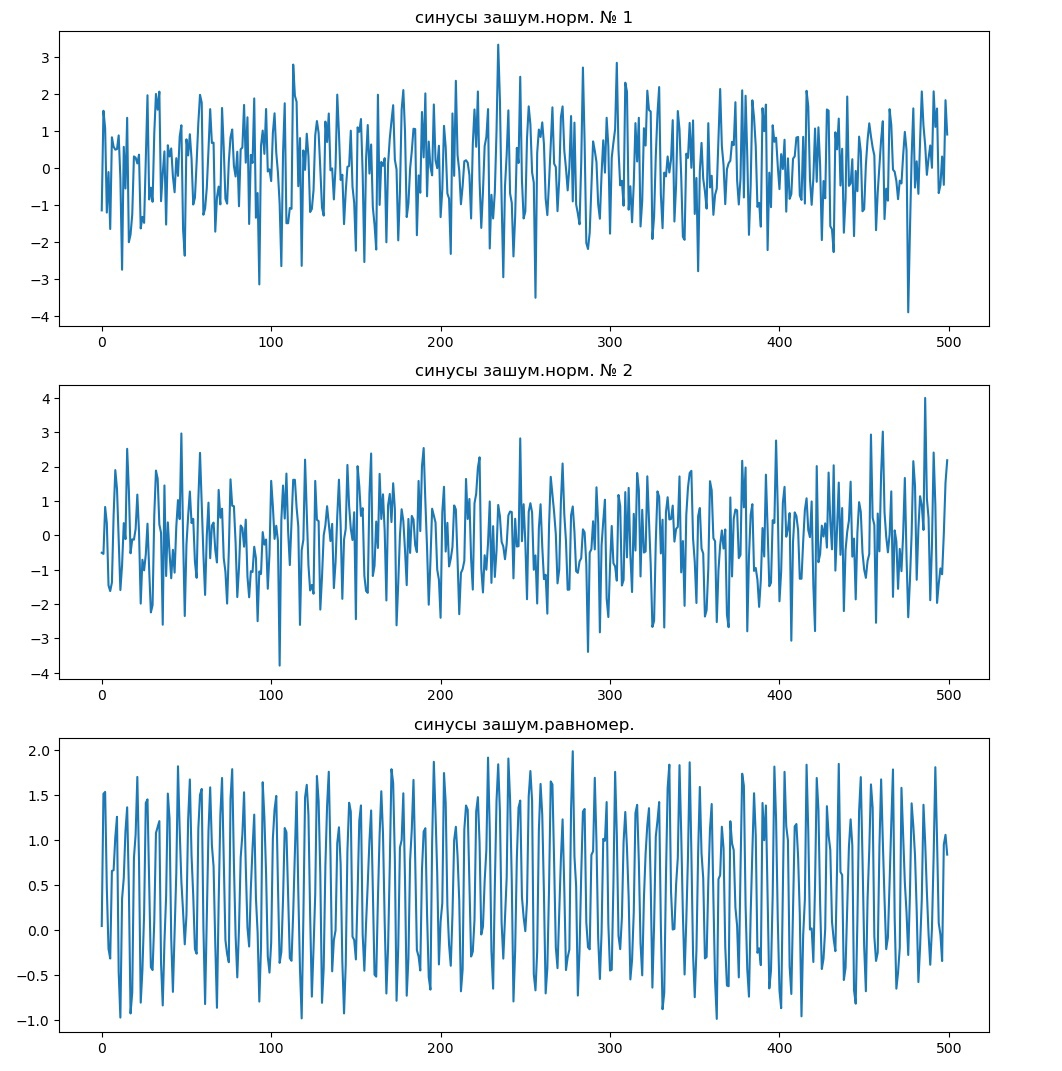
\includegraphics[width=10cm]{1}
    \caption{синусы}
    \label{fig:galaxy}
\end{figure}

   \par Таким образом явное выражение $n$-ого члена временного ряда выражается по формуле:
   \begin{equation}
       X_n = sin(n) + \xi_n 
   \end{equation}
   \par --- где $\xi_n \sim \mathcal{N}(0,1)$.
   \par С помощью модели Neural SDE, реализованной библиотекой torchsde, строится прогноз продолжения полученного ряда.
   
\begin{figure}[htp]
    \centering
    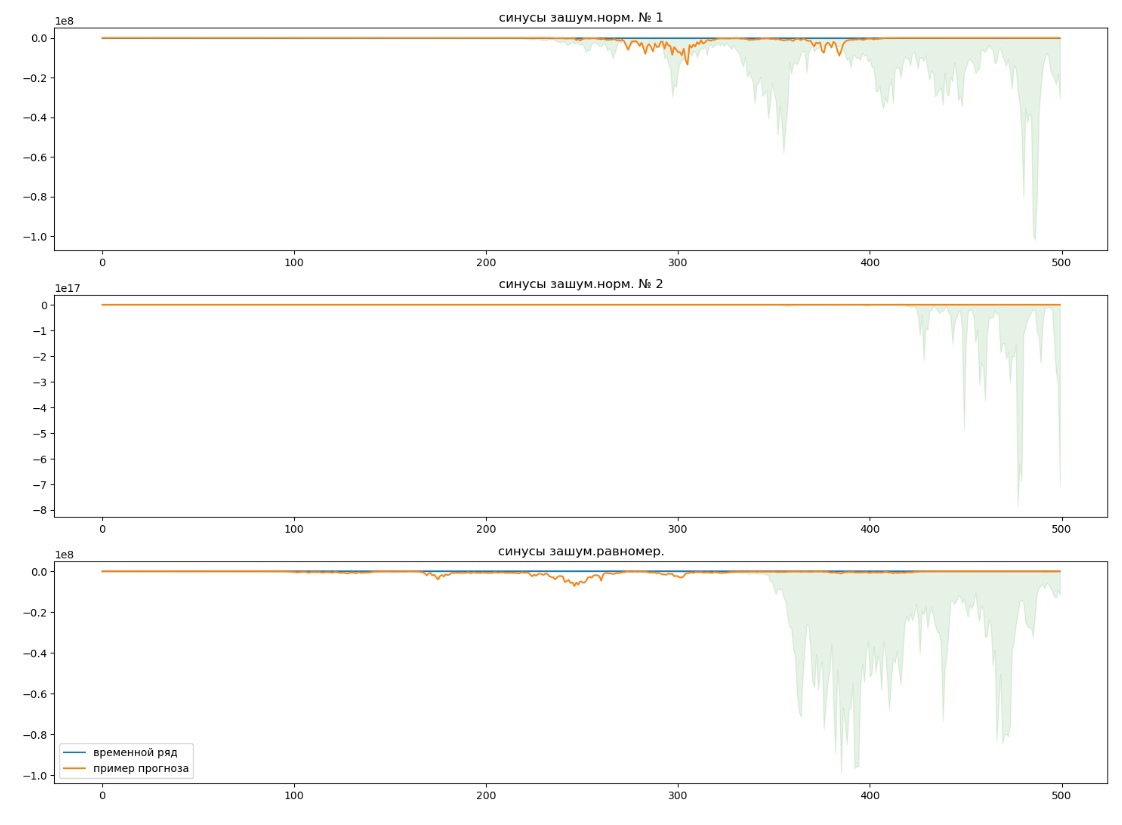
\includegraphics[width=10cm]{2}
    \caption{прогнозы SDE}
    \label{fig:galaxy}
\end{figure}
   
   \par По приращениям элементов прогноза получим матрицу фазовых траекторий процесса.
   
  \begin{figure}[t]
\centering 
\subfigure{
\label{Fig.sub.1}
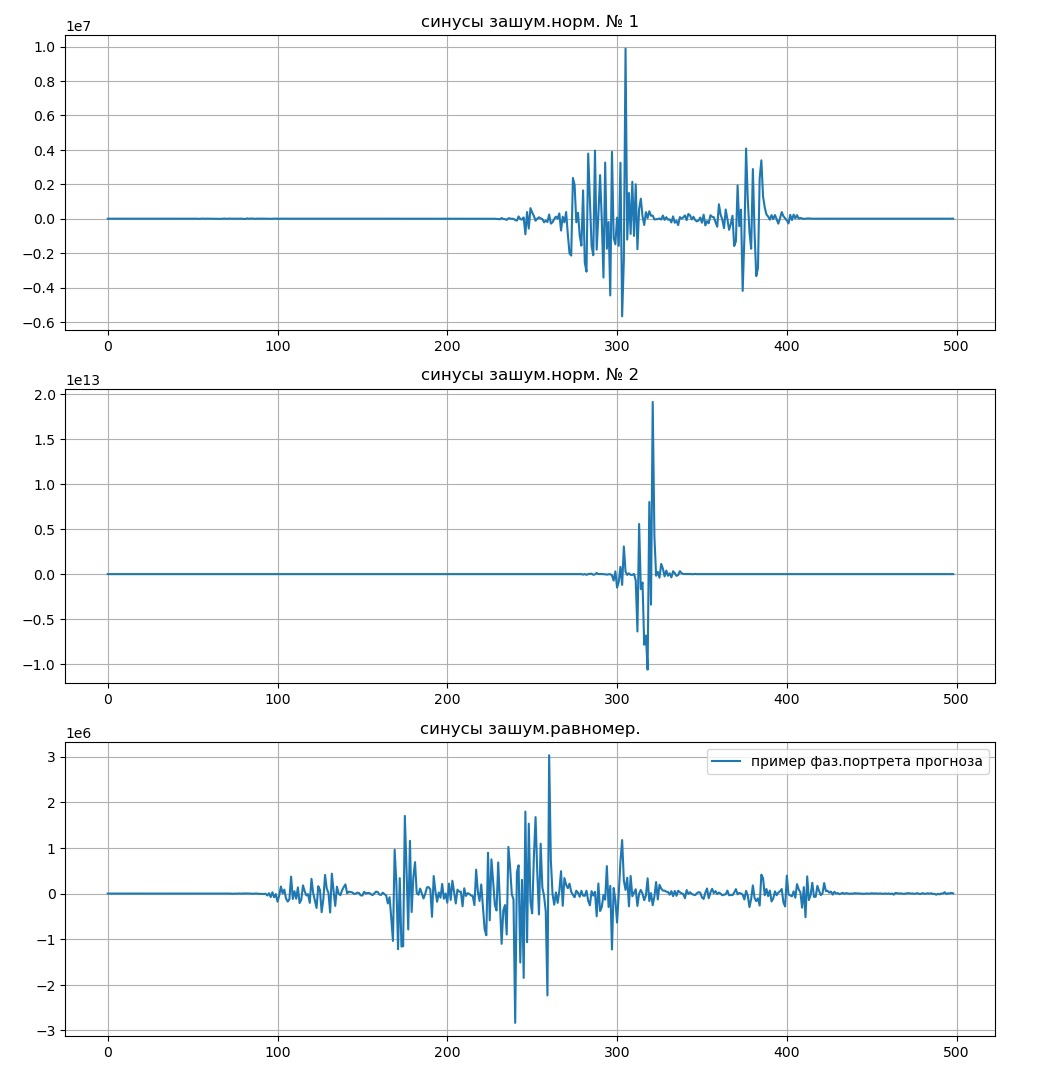
\includegraphics[width=7cm]{3}}\subfigure{
\label{Fig.sub.2}
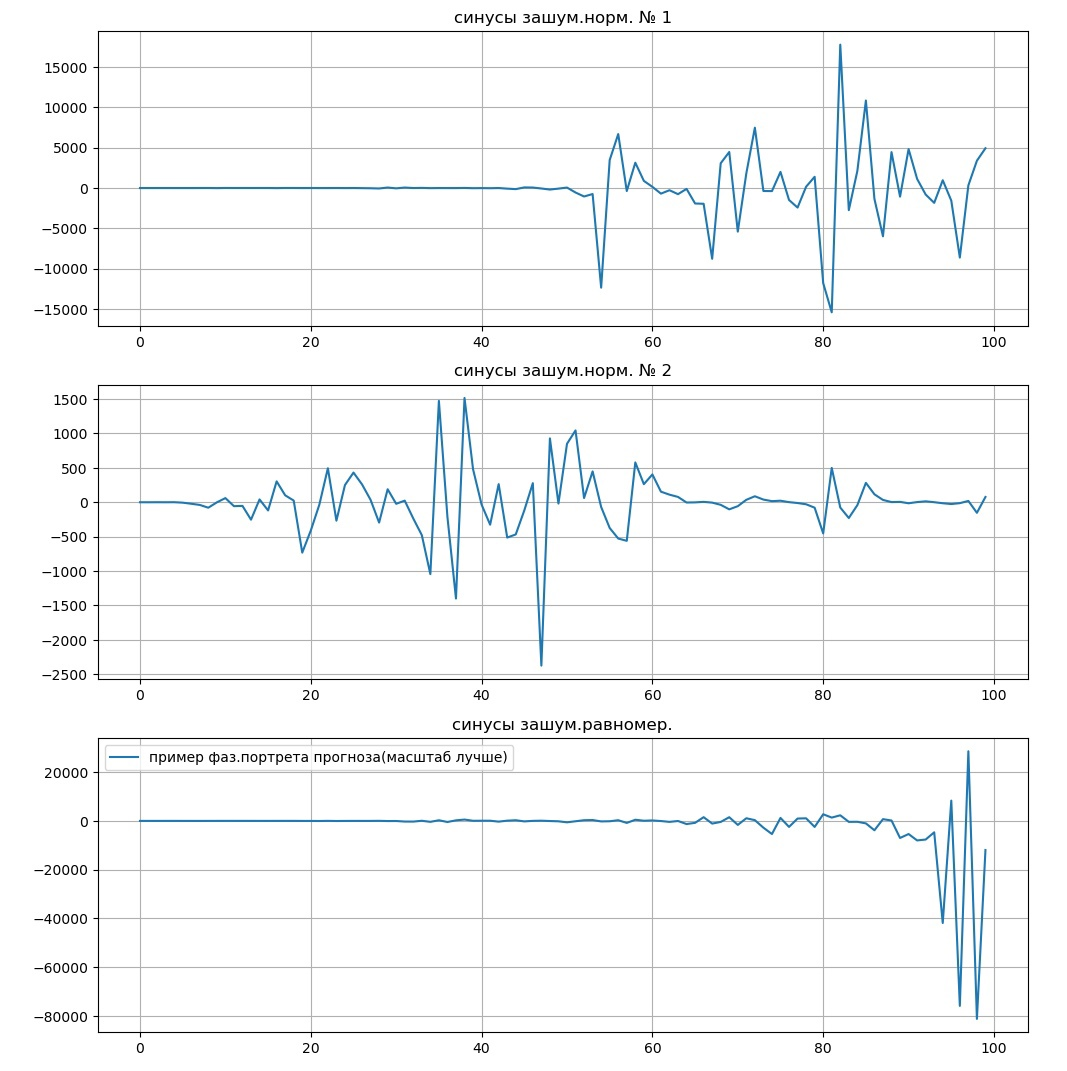
\includegraphics[width=7cm]{4}}
\caption{фазовые портреты прогнозов}
\label{1}
\end{figure}

   \par Те же шаги применимы для двух других процессов того же размера, что и $X$:
   \begin{equation}
       Y_n = sin(n) + \phi_n; \space Z_n = sin(n) + \omega_n
   \end{equation}
   \par --- где $\phi_n \sim \mathcal{N}(0,1)$, $\omega_n \sim \mathcal{U}(0,1)$.
   \par Далее, считаются $\rho_1,\rho_2$ по алгоритму, описанному в предыдущем пункте. $\rho_1$ соотвествует корреляции фазовых траекторий $X$ и $Y$, а $\rho_2$ корреляции фазовых траекторий $X$ и $Z$. Ожидается, что $|\rho_1| >> |\rho_2|$. Данный результат подтвердит верность построенного decision-rejection критерия. 

\section{Предварительный отчёт}
    

\bibliographystyle{unsrtnat}
\bibliography{references}

[1] “Neural Ordinary Differential Equations Ricky” T. Q. Chen, Yulia Rubanova, Jesse Bettencourt, David Duvenaud \\

[2] “Neural SDE: Stabilizing Neural ODE Networks with Stochastic Noise” Xuanqing Liu, Tesi Xiao, Si Si, Qin Cao, Sanjiv Kumar, Cho-Jui Hsieh  \\

[3] “Riemannian Neural SDE: Learning Stochastic Representations on Manifolds” Sung Woo Park , Hyomin Kim , Kyungjae Lee , Junseok Kwon \\

[4] “Riemannian Diffusion Models” Chin-Wei Huang, Milad Aghajohari, Avishek Joey Bose, Prakash Panangaden, Aaron Courville \\

[5] Tian Qi Chen, Yulia Rubanova, Jesse Bettencourt, and David K Duvenaud. Neural ordinary differential equations. In Advances in Neural Information Processing Systems, pages 6572–6583, 2018. \\

[6] F.Yu. Yaushev, R. V. Isachenko, V. V. Strijov. Concordant models for latent space projections in forecasting, 2020. \\

\end{document}